\subsection{$\mathrm{SE}(3) index map on $}

The index map on $\mathfrak{se}(3)$ is described below. In order to save space, we no longer deduct the index mapping in detail like $\mathfrak{so}(3)$. The index mapping on $\mathfrak{se}(3)$ is as follows:

\begin{align}
\exp \left( {{ \boldsymbol{\xi} ^ \wedge }} \right) &= \left[ {\begin{array}{*{20}{c}}
	{\sum\limits_{n = 0}^\infty {\frac{1}{{n!}}{{\left( {{\boldsymbol{\phi} ^ \wedge }} \right)}^n} } }&{\sum\limits_{n = 0}^\infty {\frac{1}{{\left( {n + 1} \right)!}}{{\left( {{\boldsymbol{\phi } ^ \wedge }} \right)}^n} \boldsymbol{\rho} } }\\
	{{\bm{0}^\mathrm{T}}}&1
	\end{array}} \right] \\
&\buildrel \Delta \over = \left[ {\begin{array}{*{20}{c}}
	\bm{R} &{\bm{J\rho} } \\
	{{\bm{0}^\mathrm{T}}}&1
	\end{array}} \right] = \bm{T}.
\end{align}

With a little patience, you can derive the $\exp$ Taylor expansion from the practice of $\mathfrak{so}(3)$. Let $\boldsymbol{\phi}=\theta \bm{a}$, where $\bm{a}$ is the unit vector, then:

\begin{equation}
	\begin{aligned}
		\sum\limits_{n = 0}^\infty {\frac{1}{{\left( {n + 1} \right)!}}{{\left( {{\boldsymbol{\phi} ^ \wedge }} \right)}^n}} &= \bm{I} + \frac{1}{{2!}}\theta {\bm{a}^ \wedge } + \frac{1}{{3 !}}{\theta ^2}{\left( {{\bm{a}^ \wedge }} \right)^2} + \frac{1}{{4!}}{\theta ^3}{ \left( {{\bm{a}^ \wedge }} \right)^3} + \frac{1}{{5!}}{\theta ^4}{\left( {{\bm{a} ^ \wedge }} \right)^4} \cdots \\
		&= \frac{1}{\theta }\left( {\frac{1}{{2!}}{\theta ^2} - \frac{1}{{4!}}{\theta ^4} + \cdots } \right)\left( {{\bm{a}^ \wedge }} \right) + \frac{1}{\theta }\left( {\frac{1}{{3!}} {\theta ^3} - \frac{1}{5}{\theta ^5} + \cdots } \right){\left( {{\bm{a}^ \wedge }} \right)^2} + \bm{I}\\
		&= \frac{1}{\theta }\left( {1 - \cos \theta } \right)\left( {{\bm{a}^ \wedge }} \right) + \frac{{\theta - \sin \theta }}{\theta }\left( {\bm{a}{\bm{a}^T} - \bm{I}} \right) + \bm{I}\\
		&= \frac{{\sin \theta }}{\theta }\bm{I} + \left( {1 - \frac{{\sin \theta }}{\theta }} \right)\bm{a }{\bm{a}^T} + \frac{{1 - \cos \theta }}{\theta }{\bm{a}^ \wedge } \buildrel \Delta \over = \bm{J}.
	\end{aligned}
\end{equation}

From the results, the $\bm{R}$ in the upper left corner of the index map of $\boldsymbol{\xi}$ is the element in the well-known $\mathrm{SO}(3)$, and $\mathfrak{se }(3)$ The rotation part of $\boldsymbol{\phi}$ corresponds. The $\bm{J}$ in the upper right corner is given by the above derivation:

\begin{equation}
\label{eq:lieAlgebraJacobian}
\bm{J} = \frac{{\sin \theta }}{\theta } \bm{I} + \left( {1 - \frac{{\sin \theta }}{\theta }} \right) \bm{a} { \bm{a}^\mathrm{T}} + \frac{{1 - \cos \theta }}{\theta }{ \bm{a}^ \wedge }.
\end{equation}

This formula is somewhat similar to the Rodrigues formula, but not exactly the same. We see that after the translation part is exponentially mapped, a linear transformation with a matrix of coefficients of $\bm{J}$ occurs. Please pay attention to the $\bm{J}$ here, as it will be used later.

Similarly, although we can also derive the logarithmic mapping analogy, there is a more trouble-free way to find the corresponding vector on $\mathfrak{so}(3)$ according to the transformation matrix $\bm{T}$: from the upper left corner $\bm{R}$ calculates the rotation vector, while $\bm{t}$ in the upper right corner satisfies:

\begin{equation}
	\bm{t} = \bm{J} \boldsymbol{\rho}.
\end{equation}

Since $\bm{J}$ can be obtained from $\boldsymbol{\phi}$, $\boldsymbol{\rho}$ can also be solved by this linear equation. Now, we have clarified the definition of Li group and Lie algebra and their mutual conversion relationship, as summarized in \autoref{fig:liegroupandAlgebra}~. If the reader doesn't understand anything, you can turn back to a few pages to see the formula derivation.

\begin{figure}[!ht]
	\centering
	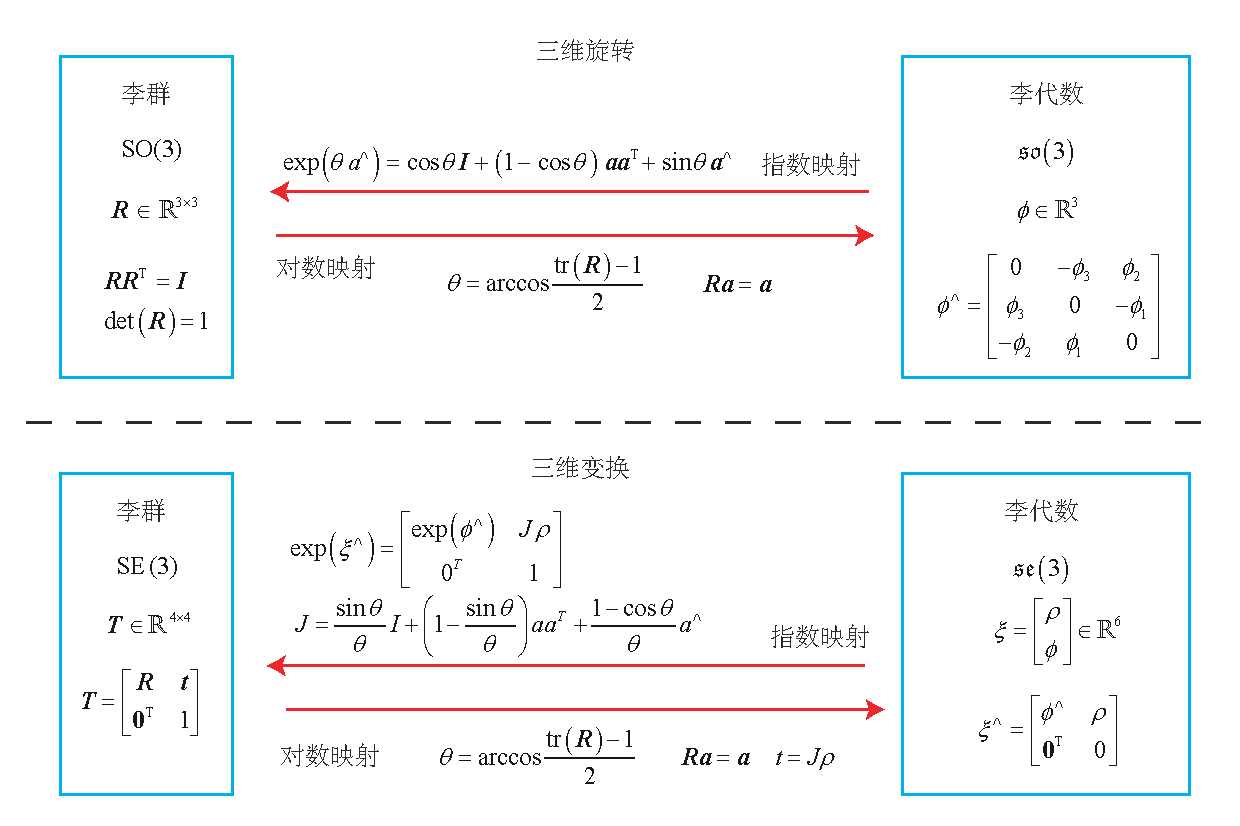
\includegraphics[width=1.0\textwidth]{chapter05/lieGroup/liegroupandAlgebra.pdf}
	The correspondence between \caption{$\mathrm{SO}(3), \mathrm{SE}(3), \mathfrak{so}(3), \mathfrak{se}(3)$. }
	\label{fig:liegroupandAlgebra}
\end{figure}

\clearpage